\icode{E-MCC-CA-L3-261024-001}
如图所示，正方形光滑玻璃板\(abcd\)水平固定放置，玻璃板距地面的高度为\(H =\)\,\qty{5.625}{m}，玻璃板正中间有一个光滑的小孔\(O\)，一根细线穿过小孔，两端分别系着小球\(A\)和小球\(B\)，小球\(A\)的质量为\qty{1}{kg}，使小球\(A\)在玻璃板上绕\(O\)点做匀速圆周运动，同时使小球\(B\)做圆锥摆运动，小球\(A\)做圆周运动的线速度大小为\qty{2}{m/s}，角速度大小为\qty{4}{rad/s}，\(OB\)悬线与竖直方向的夹角为\qty{60}{\degree}，\(A\)、\(B\)做圆周运动的周期相同，重力加速度\(g\)取\qty{10}{m/s}，不计空气阻力。求：
\begin{enumerate}
	\item 细线上的拉力的大小；
	\item 小球\(B\)的质量及连接\(A\)、\(B\)的细线的长度；
	\item 某时刻细线断开，小球\(B\)落地时的位置离\(O\)点的水平距离。
\end{enumerate}

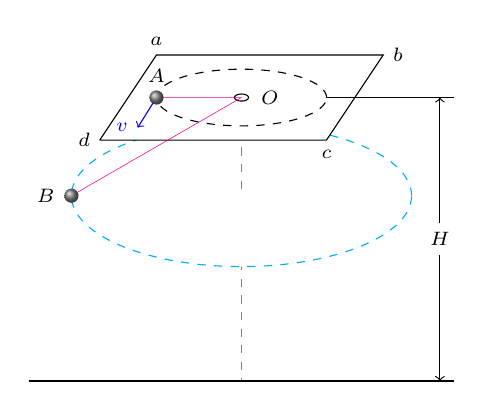
\begin{tikzpicture}[scale=.9,font=\scriptsize]
	\draw[dashed,cyan] (0,{-.8*sqrt(3)})--(0,-4);
	\draw[dashed,cyan,fill=white] (0,{-.8*sqrt(3)}) ellipse(2.4 and 1);
	\draw[dashed,cyan] (0,0)--(0,{-.8*sqrt(3)});
	\draw[fill=white] (-2,-.6)node[left]{ \(d\)}--++(3.2,0)node[below]{ \(c\)}--++(.8,1.2)node[right]{ \(b\)}--++(-3.2,0)node[above]{ \(a\)}--(-2,-.6);
		\draw (0,0)--(3,0);
	\draw[->,blue] (-1.2,0)--++(-122:.5)node[left]{\(v\)};
		\draw[fill=white,dashed] (0,0) ellipse(1.2 and .4);
	\draw (0,0) ellipse(.1 and .05);
	\draw[very thin,magenta] (-1.2,0)--(0,0)--(-2.4,{-.8*sqrt(3)});
	\shade[ball color=gray] (-2.4,{-.8*sqrt(3)}) circle(.1);
	\shade[ball color=gray] (-1.2,0) circle(.1);
	\draw[<->] (2.8,0)--node[fill=white]{ \(H\)}(2.8,-4);
	\draw[thick] (-3,-4)--(3,-4);
	\node at(-2.5,{-.8*sqrt(3)})[left]{ \(B\)};
	\node at(-1.2,.3){ \(A\)};
	\node at(.4,0){ \(O\)};
\end{tikzpicture}
\begin{answer}
    
\end{answer}